\section{Matching subtrees}
\label{sct_match}

\match{} tries to match a (smaller) "pattern" tree to the target tree(s). If
the pattern matches the target, the target tree is printed. This is typically
used to select trees that match a certain structure. For example, file
\texttt{hominoidea.nw} contains seven trees corresponding to successive
theories about the phylogeny of apes (these were taken from
\url{http://en.wikipedia.org/wiki/Hominoidea}. Let us see which of them group
humans and chimpanzees as a sister clade of gorillas (which is the current
hypothesis).

Here are small images of each of the tree in \texttt{hominoidea.nw}: \\
\bigskip{} \\
\begin{tabular}{cc}
1 (until 1960) & 2 (Goodman, 1964) \\
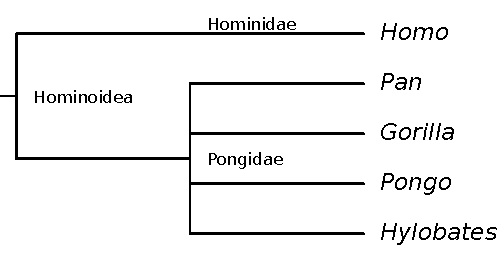
\includegraphics[scale=0.7]{homino_0.pdf} & 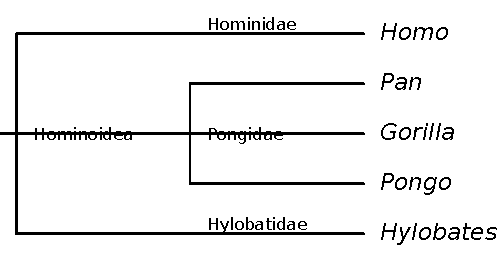
\includegraphics[scale=0.7]{homino_1.pdf} \\
3 (gibbons as outgroup) & 4 (Goodman, 1974: orangs as outgroup) \\
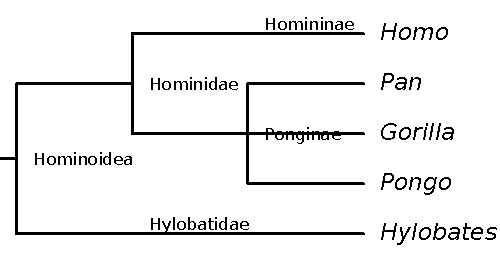
\includegraphics[scale=0.7]{homino_2.pdf} & 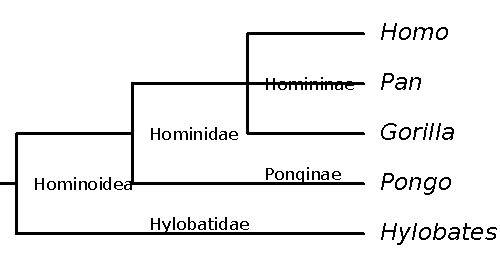
\includegraphics[scale=0.7]{homino_3.pdf} \\
5 (resolving trichotomy) & 6 (Goodman, 1990: gorillas as outgroup) \\
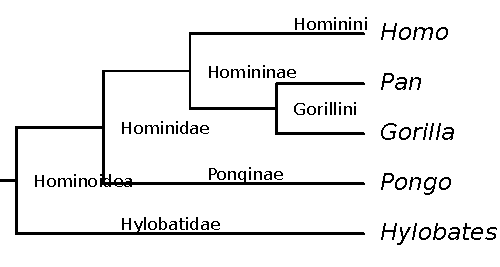
\includegraphics[scale=0.7]{homino_4.pdf} & 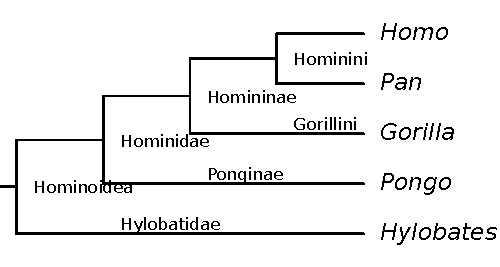
\includegraphics[scale=0.7]{homino_5.pdf} \\
7 (split of \emph{Hylobates}) \\
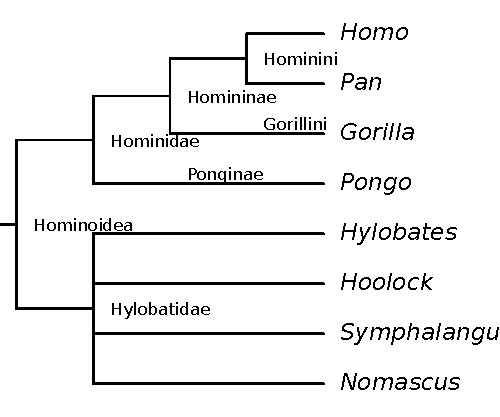
\includegraphics[scale=0.7]{homino_6.pdf} & 
\end{tabular}

\noindent{}Trees \#6 and \#7 match our criterion, the rest do not. To look for matching trees in \texttt{hominoidea.nw}, we pass the pattern on the command line:

\verbatiminput{match_1_txt.cmd}
\verbatiminput{match_1_txt.out}

\noindent{}Note that only the pattern tree's topology matters: we would get the
same results with pattern \texttt{((Homo,Pan),Gorilla);},
\texttt{((Pan,Homo),Gorilla);}, etc., but not with
\texttt{((Gorilla,Pan),Homo);} (which would select trees \#1, 2, 3, and 5. In
future versions I might add an option for strict matching.

The behaviour of \match{} can be reversed by passing option \texttt{-v} (like
\texttt{grep -v}): it will print trees that \emph{do not} match the pattern.
Finally, note that \match{} only works on leaf labels (for now), and assumes
that labels are unique in both the pattern and the target tree.
